\ifdefined\compileall \else
\ifdefined\compiletype
	\documentclass[handout]{beamer}
\else
	\documentclass{beamer}
	\def\compiletype{livebeamer}
\fi

\usepackage{templates/beamerthemekitwide}

\usepackage[utf8]{inputenc}
\usepackage[T1]{fontenc}
\usepackage[ngerman]{babel}
\usepackage{listings}
\usepackage{hyperref}
\usepackage{graphicx}

\usepackage{amsmath}
\usepackage{amsthm}
\usepackage{amssymb}
\usepackage{polynom}

\usepackage{ifthen}
\usepackage{adjustbox} % for \adjincludegraphics

\newcommand{\markBlue}[1]{\textcolor{kit-blue100}{#1}}
\newcommand{\markGreen}[1]{\textcolor{kit-green100}{#1}}

\newcommand{\pitem}{\pause\item}
\newcommand{\p}{\pause}

% -- MATH MACROS
\newcommand{\thistheoremname}{}
\newcommand{\G}{\mathbb{Z}}
\newcommand{\B}{\mathbb{B}}
\newcommand{\R}{\mathbb{R}}
\newcommand{\N}{\mathbb{N}}
\newcommand{\Q}{\mathbb{Q}}
\newcommand{\C}{\mathbb{C}}
\newcommand{\Z}{\mathbb{Z}}
\newcommand{\F}{\mathbb{F}}
\newcommand{\mi}{\mathrm{i}}
\renewcommand{\epsilon}{\varepsilon}


\newenvironment<>{taskblock}[1]{%
	\setbeamercolor{block title}{fg=kit-orange15,bg=kit-orange100}
	\setbeamercolor{block body}{fg=black,bg=kit-orange30}%
	\begin{block}#2{#1}}{\end{block}}

\setbeamertemplate{enumerate items}[default]

% Aussagenlogik Symbole
\newcommand{\W}{w}
\renewcommand{\F}{f}

% Kodierung
\newcommand{\frepr}{\textbf{repr}}
\newcommand{\fRepr}{\textbf{Repr}}
\newcommand{\fZkpl}{\textbf{Zkpl}}
\newcommand{\fbin}{\textbf{bin}}
\newcommand{\fdiv}{\textbf{ div }}
\newcommand{\fmod}{\textbf{ mod }}

\title[Grundbegriffe der Informatik]{Grundbegriffe der Informatik\\Tutorium 33}
\subtitle{}
\author{Lukas Bach, lukas.bach@student.kit.edu}
\date{\tutdate}

\institute{}

\titlelogo{lukasbach}

\titleimage{bg}
%\titleimage{bg-advent}


\ifthenelse{\equal{\compiletype}{livebeamer}}
	{
		\def\livebeamermode{1}
	}{}

\ifthenelse{\equal{\compiletype}{print}}
	{
		\def\printmode{1}
	}{}

\setbeamercovered{invisible}

%\usepackage[citestyle=authoryear,bibstyle=numeric,hyperref,backend=biber]{biblatex}
%\addbibresource{templates/example.bib}
%\bibhang1em

\begin{document}
	
\selectlanguage{ngerman}


%title page
\begin{frame}
	\titlepage
\end{frame}

%table of contents
\ifdefined\printmode
	\ifdefined\compileall \else
	\begin{frame}{Gliederung}
		\tableofcontents
	\end{frame}
\fi\fi

\fi

\section{Wiederholung}
\begin{frame}{Wiederholung}
	\pause
	
	$A := \{a, b, c\}, B := \{b, c, d\}, C := \{a, d\}$
	
	\begin{itemize}
		\pitem $A \cap B$ \pause $= \{b, c\}$
		\pitem $A \cup B$ \pause $= \{a, b, c, d\}$
		\pitem $A \backslash B$ \pause $= \{a\}$
		\pitem $C^2$ \pause $ = C \times C$ \pause $= \{(a, a), (a, d), (d, a), (d, d)\}$
		\pitem $2^C$ \pause $ = \{\emptyset$ \pause $, \{a, d\}$, \pause $\{a\}$, \pause $\{d\}\}$
		\pitem Unterschied zwischen $\{a, b\}$ und $(a, b)$?
		\pitem Definition von...
		\begin{itemize}
			\pitem Alphabet?
			\pitem Abbildung?
		\end{itemize}
	\end{itemize}
\end{frame}

\section{Wörter}

\begin{frame}{Wörter}
	\pause
	\begin{block}{Konkatenation}
		Durch Konkatenation werden einzelne Buchstaben aus einem Alphabet miteinander verbunden.
	\end{block}

	\begin{itemize}
		\pitem Symbol: $\cdot$\pause , also zwei Buchstaben $a$ und $b$ miteinander konkateniert: $a \cdot b$.
		\pitem Nicht kommutativ\pause : $a \cdot b \neq b \cdot a$
		\pitem Aber assoziativ\pause : $(a \cdot b) \cdot c = a \cdot (b \cdot c)$
		\pitem Kurzschreibweise\pause : Ohne Punkte\pause , also $a \cdot b = ab$
	\end{itemize}
\end{frame}

\begin{frame}{Wörter}
	\pause
	\begin{block}{Wörter: Intuitivere Definition}
		Ein Wort $w$ \pause entsteht durch die Konkatenation durch Buchstaben aus einem Alphabet.
	\end{block}

	\pause Also Abfolge von Zeichen.

	\pause Sei $A := \{a, b, c\}$.

	\begin{itemize}
		\pitem Mögliche Worte: \pause $w_1 := a \cdot b$\pause , $w_2 = b \cdot c \cdot c$\pause , $w_3 = a \cdot c \cdot c \cdot b \cdot a$.
		\pitem Keine möglichen Worte: \pause $d$.
		\pitem Konkatenation nicht kommutativ\pause : Wort $abc$ \pause ist ungleich dem Wort $bca$.
	\end{itemize}
\end{frame}

\begin{frame}{Wörter}
	\pause
	\begin{block}{Wörter: Abstraktere Definition}
		Ein Wort $w$ \pause über dem Alphabet $A$ \pause ist definiert als surjektive Abbildung \pause $w : \Z_n \rightarrow A$. \pause Dabei heißt $n$ \pause die Länge $|w|$ des Wortes.
	\end{block}

	\begin{itemize}
		\pitem $\Z_n$ \pause $ = \{i \in \N : \pause 0 \leq i < n \}$
		
		\pause $\Z_3 \pause = \{0, 1, 2\}, \pause \Z_2 = \{0, 1\}, \Z_0 = \emptyset$.
		
		\pitem Länge oder Kardinalität eines Wortes: \pause $|w|$. \pause $|abcde|$ \pause $= 5$.
		
		\pitem Wort $w = abdec$ als Relation aufgeschrieben: \pause $w = \{(0, a), (1, b), (2, d), (3, e), (4, c)\}$. \pause Also $w(0) = a, w(1) = b, w(2) = d, \dots$
		
		\pause Damit sieht man auch: $|w| = |\{(0, a), (1, b), (2, d), (3, e), (4, c)\}| = 5$.
	\end{itemize}
\end{frame}

\begin{frame}{Wörter}
	\pause
	\begin{itemize}
		\item Wort der Kardinalität 0?
	\end{itemize}

	\pause

	\begin{block}{Das leere Wort}
		Das leere Wort \pause $\varepsilon$ \pause ist definiert ein Wort mit Kardinalität 0\pause , also mit 0 Zeichen.
	\end{block}

	\begin{itemize}
		\pitem Leere Wort wird interpretiert als ``nicht sichtbar'' und kann überall platziert werden\pause : $aabc \pause = a\epsilon abc = \epsilon\epsilon a\epsilon bc \epsilon$.
		\pitem $|\{\epsilon\}|$ \pause $ = 1$\pause , die Menge ist nicht leer! \pause Das leere Wort ist nicht \emph{nichts}! \pause (Vergleiche leere Menge)
		\pitem $|\epsilon| = 0$.
	\end{itemize}
\end{frame}

\begin{frame}{Mehr über Wörter}

	\pause
	
	\begin{block}{$A^n$}
		Zu einem Alphabet $A$ \pause ist $A^n$ definiert als die Menge aller Wörter \pause der Länge $n$ \pause über dem Alphabet $A$.
	\end{block}

	\begin{itemize}
		\pitem Nicht mit Mengenpotenz verwechseln!
		\pitem $A := \{a, b, c\}$\pause , $A^2 = \pause \{aa, ab, ac, ba, bb, bc, ca, cb, cc\}$. \pause $A^1 \pause = A, \pause A^0 = \{\epsilon\}$.
	\end{itemize}
	
	\pause Die Menge aller Wörter \pause \emph{beliebiger} Länge: \pause
	\begin{itemize}
		\item $A^* := \bigcup_{i \in \N_0} A_i$
		\pitem $A := \{a, b, c\}$\pause . $aa \in A^*\pause , abcabcabc \in A^*\pause , aaaa \in A^*\pause , \epsilon \in A^*$.
	\end{itemize}
\end{frame}

\begin{frame}{Mehr über Wörter}
	
	\pause
	
	Konkatenation von Wörtern:
	
	\begin{itemize}
		\pitem $lager \cdot regal$ \pause $ = lagerregal$
		\pitem $lag \cdot erregal = lagerregal$
	\end{itemize}
	
	\pause
	
	\begin{block}{Konkatenation von Wörtern.}
		\begin{align*}
		w_1\cdot w_2 : \Z_{m+n} &\rightarrow A_1\cup A_2 \\
		i & \mapsto \begin{cases}
		w_1(i) & \text{ falls } 0\leq i<m \\
		w_2(i-m) & \text{ falls } m \leq i<m+n
		\end{cases}
		\end{align*}
	\end{block}

	\pause
	
	\begin{itemize}
		\item Warum $\Z_{m+n}$? \pause Wörter $w_1$ und $w_2$ \pause mit $|w_1| = m$ und $|w_2| = n$ werden konkateniert\pause , also neues Wort hat Länge $m + n$.
	\end{itemize}

\end{frame}

\begin{frame}{Mehr über Wörter}
	
	\begin{block}{Konkatenation von Wörtern.}
		\begin{align*}
		w_1\cdot w_2 : \Z_{m+n} &\rightarrow A_1\cup A_2 \\
		i & \mapsto \begin{cases}
		w_1(i) & \text{ falls } 0\leq i<m \\
		w_2(i-m) & \text{ falls } m \leq i<m+n
		\end{cases}
		\end{align*}
	\end{block}

	\pause
	
	\begin{center}
	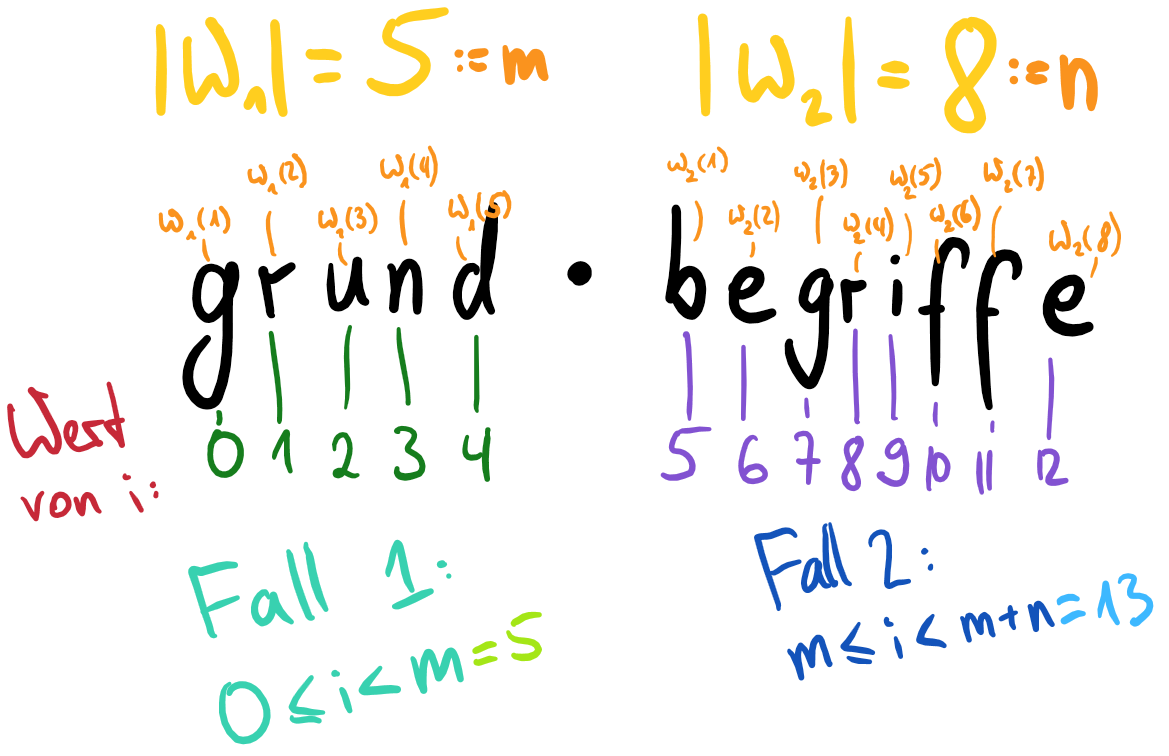
\includegraphics[width=.6\linewidth]{images/wortkonkatenation.png}
	\end{center}

\end{frame}

\begin{frame}{Mehr über Wörter}
	\begin{itemize}
		\pitem Immernoch: \pause Reihenfolge ist wichtig! \pause $OTT \cdot O = OTTO \pause \neq OOTT = O \cdot OTT$
		\pitem Auf wieviele Weisen kann man $abc$ als Konkatenation nichtleerer Wörter schreiben? \pause $abc$\pause , $a \cdot bc$\pause , $ab \cdot c$\pause , $a \cdot b \cdot c$. 
		\pitem Wortkonkatenation mit dem leeren Wort\pause : $w \cdot \epsilon$ \pause $ = w$ \pause $ = \epsilon \cdot w$.
	\end{itemize}
\end{frame}

\begin{frame}{Mehr über Wörter}
	\pause
	
	\begin{block}{Wort Potenzen}
		Sich direkt wiederholende Teilworte kann man als Wortpotenz darstellen\pause , daher $w_i^n = w_i \cdot w_i \cdots w_i$ (n $\times$ mal).
	\end{block}

	\begin{itemize}
		\pitem $a^4 = aaaa$\pause , $b^3 = bbb$\pause , $c^0 = \pause \epsilon$\pause , $d^1 = \pause d$.
		\pitem $a^3c^2b^6 \pause = aaaccbbbbbb$.
		\pitem $b \cdot a \cdot (n \cdot a)^2$ \pause $ = banana$.
		\pitem $(a^3b^2)^2c(a^2bcb^3)^3dd$ \pause $=(aaabb)^2c(aabcbbb)^3dd$ \pause $ = aaabb \cdot aaabb \cdot \quad c \quad \cdot aabcbbb \cdot aabcbbb \cdot aabcbbb \cdot \quad dd$.
	\end{itemize}
\end{frame}

\begin{frame}{Übung zu Wörter}
	Sei $A$ ein Alphabet.
	
	\begin{taskblock}{Übung zu Wörter}
		\begin{enumerate}
			\item Finde Abbildung $f: A^* \rightarrow A^*$, sodass für alle $w \in A^*$ gilt: \\\quad $2 \cdot |w| = |f(w)|$.
			\item Finde Abbildung $g: A^* \rightarrow A^*$, sodass für alle $w \in A^*$ gilt: \\\quad $|w| + 1 = |g(w)|$.
			\item Finde Abbildung $h: A^* \rightarrow A^*$, sodass für alle $w \in A^*$ gilt: \\\quad $\lfloor \frac{|w|}{2}\rfloor = |h(w)|$. (Zusatz)
			\item Sind $f, g, h$ injektiv und/oder surjektiv?
		\end{enumerate}
	\end{taskblock}

	\pause
	
	\begin{enumerate}
		\item $f: A^* \rightarrow A^*, w \mapsto w \cdot w$.
		\pitem $g: A^* \rightarrow A^*, w \mapsto w \cdot x, x \in A$.
		\pitem $h: A^* \rightarrow A^*, w \mapsto \hat{w}$ mit $ \hat{w}_i = 
			\left\{
			\begin{array}{ll}
			w_i  & \mbox{wenn } i \leq \lfloor\frac{|w|}{2}\rfloor \\
			\epsilon & \mbox{sonst }
			\end{array}
			\right\}
		$ und $i \in \Z_{|w|}$.
	\end{enumerate}
\end{frame}

\begin{frame}{Übung zu Wörter}
	\begin{enumerate}
		\item $f: A^* \rightarrow A^*, w \mapsto w \cdot w$.
		\begin{itemize}
			\pitem $f$ ist injektiv\pause , denn jedes $w$ aus der Bildmenge wird von maximal einem Wort abgebildet.
			\pitem $f$ ist nicht surjektiv\pause , denn z.B. bildet nichts auf $x \in A$ ab (oder auf andere Wörter mit ungerader Anzahl an Buchstaben).
		\end{itemize}
		\pitem $g: A^* \rightarrow A^*, w \mapsto w \cdot x, x \in A$.
		\begin{itemize}
			\pitem $g$ ist injektiv.
			\pitem $g$ ist nicht surjektiv\pause , denn z.B. bildet nichts auf $\epsilon$ ab.
		\end{itemize}
		\pitem $h: A^* \rightarrow A^*, w \mapsto \hat{w}$ mit $ \hat{w}_i = 
		\left\{
		\begin{array}{ll}
		w_i  & \mbox{wenn } i \leq \lfloor\frac{|w|}{2}\rfloor \\
		\epsilon & \mbox{sonst }
		\end{array}
		\right\}
		$ und $i \in \Z_{|w|}$.
		\begin{itemize}
			\pitem $h$ ist nicht injektiv\pause , denn z.B. $x = h(xy) = h(xz)$ mit $x,y,z \in A$.
			\pitem $h$ ist surjektiv\pause , denn für jedes $w \in A^*$ existiert ein $\hat{w} \in A^*$ mit $\hat{w} = w \cdot w$ sodass $h(\hat{w}) = w$.
		\end{itemize}
	\end{enumerate}
\end{frame}

\section{Formale Sprachen}

\begin{frame}{Formale Sprache}
	\begin{itemize}
		\pitem Was war nochmal $A^*$? Menge aller Wörter \emph{beliebiger} Länge über Alphabet $A$.
	\end{itemize}

	\pause
	
	\begin{block}{Formale Sprache}
		Eine Formale Sprache $L$ \pause über einem Alphabet $A$ ist eine Teilmenge $L \subseteq A^*$.
	\end{block}

	\begin{itemize}
		\pitem Zufälliges Beispiel: \pause $A := \{b, n, a\}$.
		\begin{itemize}
			\pitem $L_1 := \{ban, baan, nba, aa\}$ ist eine mögliche formale Sprache über $A$.
			\pitem $L_2 := \{banana, bananana, banananana, ...\}$ \pause $ = \{w : w = bana(na)^k, k \in \N\}$ auch.
			\pitem $L_3 := \{ban, baan, baaan, ...\}$ auch. \pause Andere Schreibweise? \pause \\ $ L_3 = \{w : w = ba^kn, k \in \N \}$
		\end{itemize}
		\pitem Formale Sprachen sind also nicht zwangsweise endliche Mengen.
		\pitem Praktischeres Beispiel: $A := \{w : w $ ist ein ASCII Symbol $\}$.
		\begin{itemize}
			\pitem $L_4 := \{class, if, else, while, for, ...\}$ ist eine formale Sprache über $A$.
			\pitem $L_5 := \{w : w = a \cdot b$ mit $a$ als Großbuchstabe und $b$ als Groß- oder Kleinbuchstabe $ \} \pause \backslash L_4$ \pause ist eine formale Sprache von korrekten Klassennamen in Java.
		\end{itemize}
	\end{itemize}
\end{frame}

\begin{frame}{Übung zu formalen Sprachen}
	\pause
	
	$A := \{a, b\}$
	
	\begin{itemize}
		\pitem Sprache $L$ aller Wörter über $A$, die nicht das Teilwort $ab$ enthalten?
		\begin{itemize}
			\pitem Was passiert wenn ein solches Wort ein $a$ enthält? \pause Dann keine $b$'s mehr!
			\pitem $L = \{w_1 \cdot w_2 : w_1 \in \{b\}^*$ und $w_2 \in \{a\}^* \}$
			\pitem Andere Möglichkeit\pause : Suche Wörter mit $ab$ und nehme diese Weg.
			\pitem $L = \{a, b\}^*\pause \backslash\{ w_1 \cdot ab \cdot w_2 : w_1, w_2 \in \{a,b\}^* \}$
		\end{itemize}
	\end{itemize}
\end{frame}

\begin{frame}{Übung zu formalen Sprachen}
	
	Sei $A := \{a, b\}, B := \{0, 1\}$.
	
	\begin{taskblock}{Aufgabe zu formalen Sprachen}
		\begin{enumerate}
			\item Sprache $L_1 \subseteq A^*$ von Wörtern, die mindestens drei $b$'s enthalten.
			\item Sprache $L_2 \subseteq A^*$ von Wörtern, die gerade Zahl von $a$'s enthält.
			\item Sprache $L_3 \subseteq B^*$ von Wörtern, die, interpretiert als Binärzahl eine gerade Zahl sind.
		\end{enumerate}
	\end{taskblock}

	\pause
	
	\begin{enumerate}
		\item $L_1 \pause = \{w = w_1  b  w_2  b  w_3 b w_4 : w_1,w_2,w_3,w_4 \in A^* \}$
		\pitem $L_2 \pause = \{w = (w_1 a w_2 a w_3)^* : w_1,w_2,w_3 \in \{b\}^* \}$ \pause (Ist da $\epsilon$ drin?)
		\pitem $L_3 \pause = \{w = w \cdot 0 : w \in B^* \}$
	\end{enumerate}
\end{frame}

\ifdefined\compileall
\else


\ifthenelse{\equal{\compiletype}{print}}
{

\begin{frame}{Informationen}
	
	\begin{columns}
		\begin{column}{0.5\textwidth}
			
			\begin{block}{Zum Tutorium}
				\begin{itemize}
					\item Lukas Bach
					\item Tutorienfolien auf: 
					\begin{itemize}
						\item \url{http://gbi.lukasbach.com}
					\end{itemize}
					\item Tutorium findet statt:
					\begin{itemize}
						\item Donnerstags, 14:00 - 15:30
						\item 50.34 Informatikbau, -107
					\end{itemize}
				\end{itemize}
			\end{block}
			
			\begin{block}{Mehr Material}
				\begin{itemize}
					\item Ehemalige GBI Webseite:
					\begin{itemize}
						\item \url{http://gbi.ira.uka.de}
						\item Altklausuren!
					\end{itemize}
				\end{itemize}
			\end{block}
			
		\end{column}
		\begin{column}{0.5\textwidth}
			
			\begin{block}{Zur Veranstaltung}
				\begin{itemize}
					\item Grundbegriffe der Informatik
					\item Klausurtermin:
					\begin{itemize}
						\item 06.03.2017, 11:00
						\item Zwei Stunden Bearbeitungszeit
						\item 6 ECTS für Informatiker und Informationswirte, 4 ECTS für Mathematiker und Physiker
					\end{itemize}
				\end{itemize}
			\end{block}
			
			\begin{block}{Zum Übungsschein}
				\begin{itemize}
					\item Übungsblatt jede Woche
					\item Ab 50\% insgesamt hat man den Übungsschein
					\item Keine Voraussetzung für die Klausur, aber für das Modul
				\end{itemize}
			\end{block}
			
		\end{column}
	\end{columns}
	
\end{frame}

}{}

\ifdefined\livebeamermode
	\begin{frame}
		
\includegraphics[width=\linewidth]{images/thatsall.png}
	\end{frame}
\fi

\end{document}

\fi